\section{Calibration and Estimation}
\label{sec:calibration_and_estimation}

The model is described by a large number of parameters that govern the number of
contacts a person has, the likelihood of becoming infected on each contact, the
likelihood of developing light or strong symptoms or even dying from the disease as well
as the duration each stage of the disease takes.

Most of these parameters can be calibrated from existing datasets or the medical
literature. Only the infection probabilities have to be estimated inside the model by
fitting it to time series data of case numbers and fatality rates.


\subsection{Medical Parameters}

This section discusses the medical parameters used in the model, their sources and how we arrived at the distributions used in the model.\footnotemark

\footnotetext{Additional information can be found in the \href{https://sid-dev.readthedocs.io/en/latest/reference_guides/epi_params.html}{online documentation}.}


\subsubsection{Length of Presymptomatic Stage / Incubation Period}


Estimates of the incubation period usually give a range from 2 to 12 days. A meta analysis by \citet{McAloon2020} comes to the conclusion that ``The incubation period distribution may be modeled with a lognormal distribution with pooled $\mu$ and $\sigma$ parameters (95\% CIs) of 1.63 (95\% CI 1.51 to 1.75) and 0.50 (95\% CI 0.46 to 0.55), respectively.'' For simplicity we discretize this distribution into four bins.


\subsubsection{Begin of Infectiousness}

The period between infection and onset of infectiousness is called latent or latency period. However, the latency period is rarely given in epidemiological reports on Covid-19. Instead, scientists and agencies usually report the incubation period, the period from infection to the onset of symptoms. A few studies used measurements of virus shedding to estimate infectiousness during the course of the disease. When measurements started before the onset of symptoms the development of the viral load before symptoms gives us an indication of number of days between the onset of infectiousness and symptoms.

The European Centre for Disease Prevention and Control estimates that people become infectious between one and two days before the symptoms set in. This is similar to \citet{He2020} who estimate this to take 2.3 days and is in line with \citet{Peak2020}.

Given these numbers and the length of the incubation period we can calculate the latency period for symptomatic people. To our knowledge no estimates for the latency period of asymptomatic cases of COVID-19 exist. We assume it to be the same for symptomatic and asymptomatic cases.

Thus, we arrive at the following distribution for latency periods: 40\% have one day. 35\% have two days. 20\% have three days and 5\% have 5 days.


\subsubsection{Duration of Infectiousness}

We assume that the duration of infectiousness is the same for both symptomatic and asymptomatic individuals as evidence suggests little differences in the transmission rates of SARS-CoV-2 virus between symptomatic and asymptomatic patients (\citet{Yin2020}) and that the viral load between symptomatic and asymptomatic individuals are similar (\citet{Zou2020}, \citet{Byrne2020}, \citet{Singanayagam2020}).

Our distribution of the duration of infectiousness is based on \citet{Byrne2020}.

For symptomatic cases they arrive at 0-5 days before symptom onset (figure 2) and 3-8 days of infectiousness afterwards.\footnote{Viral loads may be detected much later but 8 days seems to be the time after which most people are culture negative, as also reported by \citet{Singanayagam2020}} Thus, we arrive at 0 to 13 days as the range for infectiousness among individuals who become symptomatic (see also figure 5). This duration range is very much in line with the meta-analysis’ reported evidence for asymptomatic individuals (see their figure 1). Thus, we arrive at 0 to 13 days as the range for infectiousness among individuals who become symptomatic. This duration range is very much in line with the meta-analysis' reported evidence for asymptomatic individuals.

Following this evidence we assume the following discretized distribution of the infectiousness period: 10\% of individuals are infectious for three days, 25\% for five days, another 25\% for seven days, 20\% for nine days and 20\% for eleven days.


\subsubsection{Duration of Symptoms}

We use the duration to recovery of mild and moderate cases reported by \cite[Figure~S3, Panel~2]{Bi2020} for the duration of symptoms for asymptomatic and non-ICU requiring symptomatic cases.

We collapse the data to the following distribution: 10\% recover after 15 days and 30\% require 18, 22 or 27 days respectively.

These numbers are only used for mild cases. We do not disaggregate by age. Note that the length of symptoms is not very important in our model given that individuals stop being infectious before their symptoms cease.


\subsubsection{Time from Symptom Onset to Admission to ICU}

The data on how many percent of symptomatic patients will require ICU is pretty thin. We rely on data by the US CDC (\citet{Stokes2020}) and \href{https://github.com/BDI-pathogens/OpenABM-Covid19/blob/572e24ca2dbf7153789a92ad3a27e4c515d0e576/documentation/parameters/parameter_dictionary.md}{the OpenABM-Project}. Table~\ref{tab:symptomatic-to-ICU} shows our derivations for the probabilities of requiring intensive care per age group.

\begin{table}[tb]
    \caption{Shares of symptomatic patients who will require ICU care by age groups.}
    \label{tab:symptomatic-to-ICU}
    \centering

    \begin{tabular}{ll}
        \toprule
        Age Group & Share \\
        \midrule
        0-9 & 0.00005 \\
        10-19 & 0.00030 \\
        20-29 & 0.00075 \\
        30-39 & 0.00345 \\
        40-49 & 0.01380 \\
        50-59 & 0.03404 \\
        60-69 & 0.10138 \\
        70-79 & 0.16891 \\
        80-100 & 0.26871 \\
        \bottomrule
    \end{tabular}

    \tablenotes{The data is taken from \citet{Stokes2020} and \href{https://github.com/BDI-pathogens/OpenABM-Covid19/blob/572e24ca2dbf7153789a92ad3a27e4c515d0e576/documentation/parameters/parameter_dictionary.md}{the OpenABM-Project}.}

\end{table}

For those who will require intensive care we follow \citet{Chen2020} who estimate the time from symptom onset to ICU admission as 8.5 $\pm$ 4 days.

This aligns well with numbers reported for the time from first symptoms to hospitalization: \citet{Gaythorpe2020} report a mean of 5.76 with a standard deviation of 4. This is also in line with the durations collected by \href{https://www.rki.de/DE/Content/InfAZ/N/Neuartiges_Coronavirus/Steckbrief.html#doc13776792bodyText16}{the Robert Koch Institut}.

We assume that the time between symptom onset and ICU takes 4, 6, 8 or 10 days with equal probabilities. These times mostly matter for the ICU capacities.


\subsubsection{Death and Recovery from ICU}

We take the survival probabilities and time to death and time until recovery from intensive care from the \href{https://tinyurl.com/y5owhyts}{OpenABM Project}.

They report time until death to have a mean of 11.74 days and a standard deviation of 8.79 days. Approximating this with the normal distribution, we have nearly 10\% probability mass below 0. We use it nevertheless as several other distributions (such as chi squared and uniform) were unable to match the variance.
Discretizing this leads to 41\% of individuals who die from Covid-19 to die after one day in intensive care. 22\% day after 12 days, 29\% after 20 days and 7\% after 32 days. Again, we rescale this for every age group among those that will not survive.

They report time until recovery to have a mean of 18.8 days and a standard deviation of 12.21 days. Approximating this with the normal distribution, we have over 5\% probability mass below 0. Discretizing this of those who recover in intensive care 22\% do so after one day, 30\% after 15 days, 28\% after 25 days and 18\% after 45 days.


\subsection{Number of Contacts}
\label{sub:number_of_contacts}

We calibrate the parameters for the predicted numbers of contacts from contact diaries
of over 2000 individuals from Germany, Belgium, the Netherlands and Luxembourg
\citep{Mossong2008}. Each contact diary contains all contacts an individual had
throughout one day, including information on the other person (such as age and gender)
and information on the contact. Importantly, for each contact individuals entered of
which type the contact (school, leisure, work etc.) was and how frequent the contact
with the other person is.

Thus, we can use the empirical distributions from this data as pre-pandemic number of
contacts.


\FloatBarrier


\subsection{Assortative Matching}

As mentioned in section \ref{sec:matching}, the probability that two individuals are
matched can depend on background characteristics. In particular, we allow this
probability to depend on age and county of residence. While we do not have good data on
geographical assortativeness and just roughly calibrate it such that 60 \% of contacts
are within the same county, we can calibrate the age assortativeness from
the same data we use to calibrate the number of contacts.

\begin{figure}[h]
    \centering
    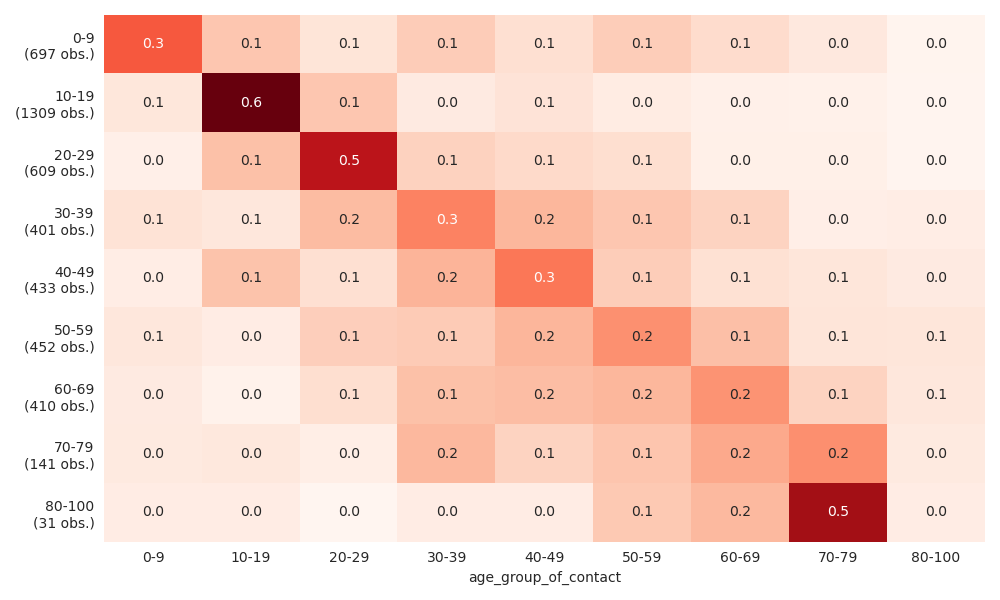
\includegraphics[width=0.9 \textwidth]{../figures/assortative_matching_probability_example.png}
    \caption{Distribution of random non-work contacts by age of participants.}
    \label{fig:assortativeness}
    \figurenotes{
        The figure shows the distribution of random non-work contacts by age groups. A
        row shows the share of contacts a certain age group has with all other age
        groups. Higher values are colored in darker red tones. The diagonal represents
        the share of contacts with individuals from the same age group.
    }
\end{figure}

Figure~\ref{fig:assortativeness} shows that assortativeness by age is especially strong
for children and younger adults. For older people, the pattern becomes more dispersed
around their own age group, but within-age-group contacts are still the most common
contacts.

\FloatBarrier


\subsection{Infection Probabilities}
\label{sec:estimation}

To calibrate infection probabilities outside of the model, it would be important to know
the exact duration and distance of each contact type as well as viral loads. Since this
is not available in any dataset, we estimate those parameters inside the model with the
method of simulated moments \citep{McFadden1989} by minimizing the distance between
simulated and observed infection rates. Since our model includes a lot of randomness, we
average simulated infection rates over several model runs.

Currently, we use data for Germany from August until November.
We do not use earlier periods to save computational time.
Moreover, we would be worried that the there are seasonal effects that we currently do
not model.

To avoid overfitting and simplify the numerical optimization problem, we only allow for
four different probabilities: 1) for contacts in schools, preschools and nurseries. 2)
for work contacts. 3) for households. 4) for leisure activities.

\subsection{Policies}

\FloatBarrier

In our empirical application we distinguish four groups of contact types:
households, education, work and other contacts.
For households we assume that the individuals' contacts in their households do not change
over our estimation period.
For nurseries, preschools and schools we implement vacations as announced by the German
federal states as well as school closures. For the moment we ignore both emergency
childcare and that lack of childcare leads working parents to stay home.
%
% Schließung von Kindertagesstätten und Schulen: 37,4 Millionen ausgefallene Arbeitstage
% http://www.iab-forum.de/schul-und-kitaschliessungen-krankheit-quarantaene-die-coronabedingten-arbeitsausfaelle-der-erwerbstaetigen-steigen-auf-592-millionen-arbeitstage/
%
%
% https://www.sueddeutsche.de/politik/schulschliessung-lockdown-bildung-1.5190377:
% In allen Ländern geht trotz des Lockdowns ein erheblicher Anteil der Schülerinnen und
% Schüler in die Schule.
% https://gfx.sueddeutsche.de/apps/e525337/www/_image_desktopw1840q70-1e2e2bf78b7d4430.png
% 18% der Grundschüler in Notbetreuung in BW
%
For our work models\footnotemark we use the reductions in work mobility reported in the
Google Mobility Data \citep{Google2021} to calibrate our work policies.
Reductions in work contacts are not random but governed through a work contact priority
where the policy changes the threshold below which workers stay home.
Figure \ref{fig:work_multiplier} shows the share of workers that go to work in our model
over time.

\begin{figure}[h]
    \centering
    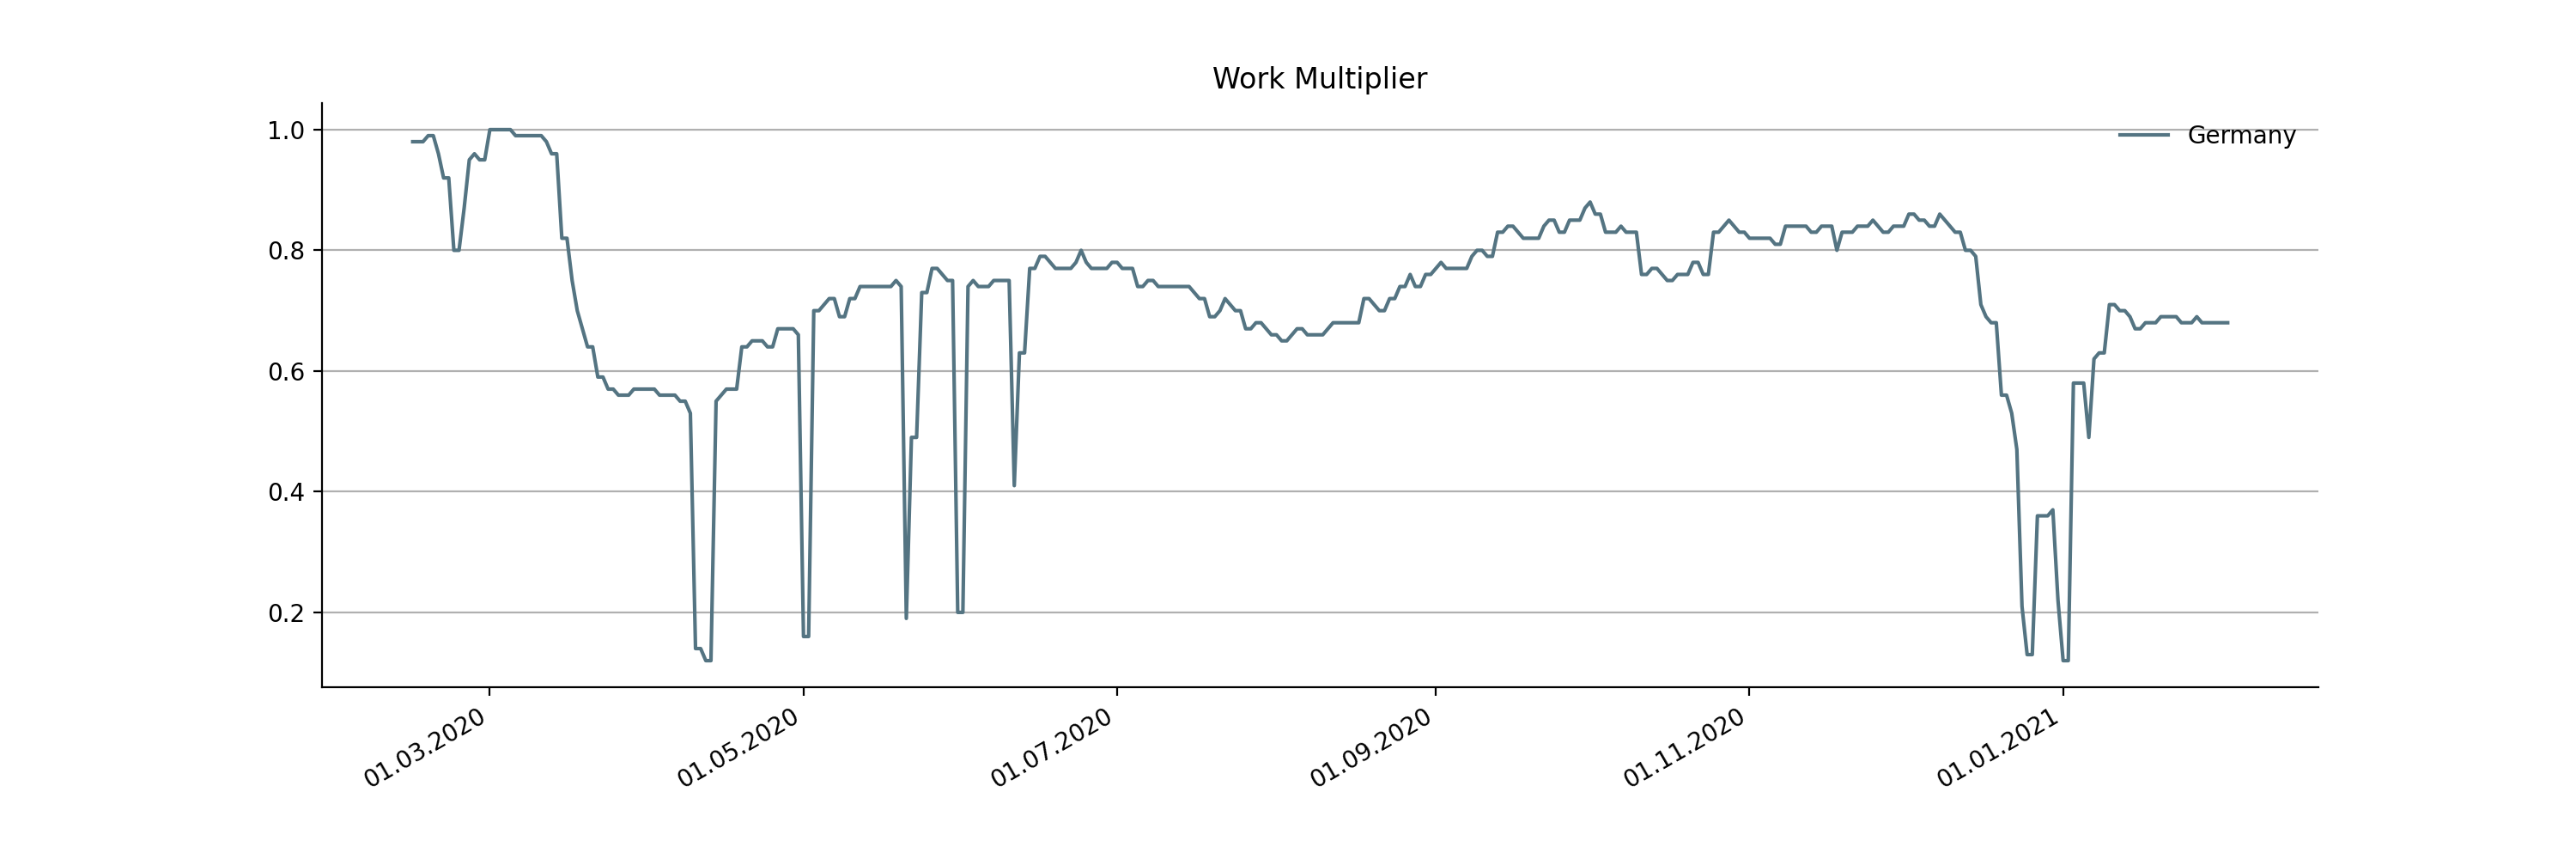
\includegraphics[width=1.1 \textwidth]{../figures/work_multiplier.png}
    \caption{Share of workers attending work normally.}
    \label{fig:work_multiplier}
    \figurenotes{
        The figure shows the percentage of pre-pandemic work mobility taking place
        since the start of the pandemic. In our model this is used as a proxy for the
        share of workers that attend work as usual. Workers are ordered with the
        importance of personal contacts for their work. Thus, if the share of
    }
\end{figure}

\footnotetext{We distinguish non-recurrent work contacts, daily work contacts and weekly work contacts.}

For the last group of contacts which cover things like leisure activities, grocery
shopping etc. we have no reliable data by how much policies reduce them.
In addition, they are likely to be affected by social and psychological factors such as
pandemic fatigue and vacations. Because of this we estimate them like the infection
probabilities to fit the time series data. We use very few change points and tie them to
particular events such as policy announcements or particular holidays.

\FloatBarrier
